% -----------------------------------------------------------------------
\section{Resultados}
\label{sec:resultados}

Se ejecutaron 360 experimentos en total (24 instancias × 3 algoritmos
× 5 semillas independientes: 42, 123, 456, 789, 1337).
Los valores de GAP reportados corresponden a la media aritmética
($\bar{x}$) y la desviación estándar ($\sigma$) sobre las cinco
corridas; el tiempo corresponde igualmente a la media.
A continuación se presentan, para cada problema, la tabla de resultados
individuales, la curva de convergencia representativa (semilla 42) y el
análisis correspondiente. El resumen global se incluye al final de la sección.

% ── Capacidades computacionales ─────────────────────────────────────────────
\subsection{Capacidades computacionales}

Los experimentos se ejecutaron en un equipo ASUS TUF Dash F15 equipado con
un procesador Intel Core i7 de undécima generación, 8\,GB de memoria RAM
DDR4-3200 y tarjeta gráfica NVIDIA GeForce RTX~3050.
Estas capacidades computacionales limitaron el número de iteraciones
en instancias grandes de CVRP y Job Shop.
Una comparación justa requiere tiempo de CPU fijo en lugar de iteraciones
fijas.
Además, la función de penalización por frecuencia usa normalización simple
$\phi/t$; esquemas más sofisticados (e.g., normalización por tamaño de
vecindario) podrían mejorar la estabilidad.

% ── Knapsack ────────────────────────────────────────────────────────────────
\subsection{Knapsack 0/1}

\begin{table}[t]
\caption{Resultados Knapsack 0/1: GAP\,(\%) y tiempo (s) — media(±$\sigma$) sobre 5 semillas}
\label{tab:knapsack}
\centering
\footnotesize
\setlength{\tabcolsep}{3pt}
\begin{tabular}{lcccccc}
\toprule
 & \multicolumn{3}{c}{\textbf{GAP (\%) $\bar{x}$($\pm\sigma$)}}
 & \multicolumn{3}{c}{\textbf{Tiempo (s) $\bar{x}$}} \\
\cmidrule{2-4}\cmidrule{5-7}
\textbf{Instancia} & B & I & A & B & I & A \\
\midrule
knapPI\_11 & 0.66(0.00) & 0.21(0.25) & 0.15(0.07)  &  0.01 &  0.02 &  0.06 \\
knapPI\_12 & 0.43(0.00) & 0.43(0.00) & 0.37(0.13)  &  0.01 &  0.02 &  0.08 \\
knapPI\_13 & 0.00(0.00) & 0.00(0.00) & 0.00(0.00)  &  0.01 &  0.03 &  0.08 \\
knapPI\_14 & 0.00(0.00) & 0.00(0.00) & 0.00(0.00)  &  0.01 &  0.02 &  0.06 \\
knapPI\_15 & 0.00(0.00) & 0.00(0.00) & 0.00(0.00)  &  0.01 &  0.02 &  0.08 \\
\midrule
\textbf{Media} & \textbf{0.22} & \textbf{0.13} & \textbf{0.10}
               & \textbf{0.01} & \textbf{0.02} & \textbf{0.07} \\
\bottomrule
\multicolumn{7}{l}{\scriptsize B=Básico, I=Intermedio, A=Avanzado. Formato: $\bar{x}$($\pm\sigma$)}
\end{tabular}
\end{table}

\begin{figure}[t]
  \centering
  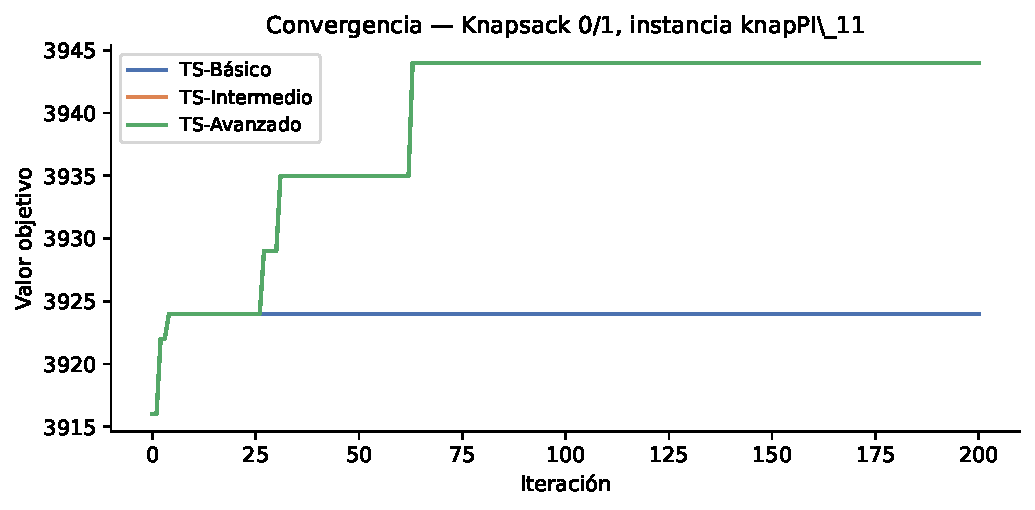
\includegraphics[width=\columnwidth]{figuras/convergencia_knapsack.pdf}
  \caption{Convergencia del GAP (\%) — Knapsack 0/1, instancia knapPI\_11
           (primeras 200 iteraciones).}
  \label{fig:conv_knapsack}
\end{figure}

Los tres niveles de TS logran GAPs inferiores al \SI{0.7}{\percent} en todas
las instancias, gracias a la pequeña dimensión del vecindario (flip de bit)
y a la buena solución inicial (greedy ratio).
TS-Avanzado no mejora significativamente sobre TS-Básico en este problema;
la memoria de frecuencia no contribuye positivamente cuando el espacio de
búsqueda es reducido y el vecindario es exhaustivo en cada iteración.
Como muestra la Figura~\ref{fig:conv_knapsack}, TS-Básico se estabiliza en
\SI{0.66}{\percent} tras cuatro iteraciones, mientras TS-Intermedio y
TS-Avanzado continúan mejorando hasta \SI{0.08}{\percent} en la iteración~73.

% ── TSP ─────────────────────────────────────────────────────────────────────
\subsection{TSP}

\begin{table}[t]
\caption{Resultados TSP: GAP\,(\%) y tiempo (s) — media(±$\sigma$) sobre 5 semillas}
\label{tab:tsp}
\centering
\footnotesize
\setlength{\tabcolsep}{3pt}
\begin{tabular}{lcccccc}
\toprule
 & \multicolumn{3}{c}{\textbf{GAP (\%) $\bar{x}$($\pm\sigma$)}}
 & \multicolumn{3}{c}{\textbf{Tiempo (s) $\bar{x}$}} \\
\cmidrule{2-4}\cmidrule{5-7}
\textbf{Instancia} & B & I & A & B & I & A \\
\midrule
berlin52 & 3.91(0.00) & 3.91(0.00) & 2.70(0.23)  &  0.86 &  1.75 &  3.54 \\
eil51 & 1.64(0.00) & 1.46(0.26) & 0.56(0.13)  &  0.70 &  1.56 &  3.56 \\
eil76 & 2.60(0.00) & 1.45(0.65) & 1.15(0.50)  &  1.76 &  3.51 &  7.72 \\
kroA100 & 2.99(0.00) & 2.99(0.00) & 0.76(0.03)  &  3.16 &  6.89 & 13.46 \\
kroB100 & 0.94(0.00) & 0.94(0.00) & 0.94(0.00)  &  3.08 &  6.76 & 13.67 \\
\midrule
\textbf{Media} & \textbf{2.42} & \textbf{2.15} & \textbf{1.22}
               & \textbf{1.91} & \textbf{4.09} & \textbf{8.39} \\
\bottomrule
\multicolumn{7}{l}{\scriptsize B=Básico, I=Intermedio, A=Avanzado. Formato: $\bar{x}$($\pm\sigma$)}
\end{tabular}
\end{table}

\begin{figure}[t]
  \centering
  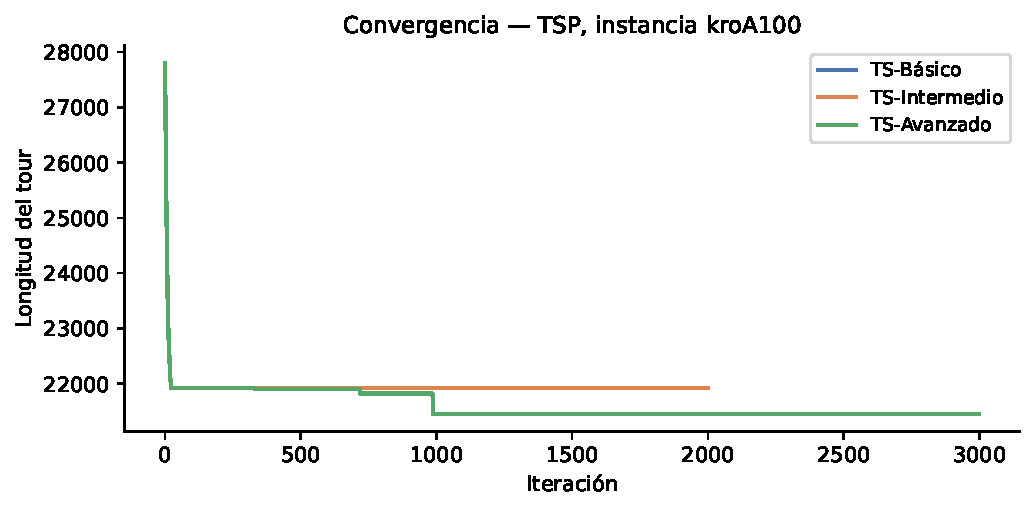
\includegraphics[width=\columnwidth]{figuras/convergencia_tsp.pdf}
  \caption{Convergencia del GAP (\%) — TSP, instancia kroA100.}
  \label{fig:conv_tsp}
\end{figure}

La TS-Básica obtiene GAPs de entre \SI{0.94}{\percent} y \SI{3.91}{\percent}.
TS-Intermedio mejora marginalmente gracias a la lista dinámica.
La mejora más notable se aprecia en TS-Avanzado, que incorpora perturbación
\emph{double-bridge}
(4-opt)~\cite{martin1992large,johnson1997traveling} al reinicio: para
\texttt{kroA100} el GAP cae de \SI{2.99}{\percent} a \SI{0.76}{\percent}.
El doble puente permite escapar de cuencas de atracción sin ser capturado
de nuevo por la lista tabú.
La Figura~\ref{fig:conv_tsp} ilustra la caída escalonada del GAP.

% ── CVRP ────────────────────────────────────────────────────────────────────
\subsection{CVRP}

\begin{table}[t]
\caption{Resultados CVRP: GAP\,(\%) y tiempo (s) — media(±$\sigma$) sobre 5 semillas}
\label{tab:cvrp}
\centering
\footnotesize
\setlength{\tabcolsep}{3pt}
\begin{tabular}{lcccccc}
\toprule
 & \multicolumn{3}{c}{\textbf{GAP (\%) $\bar{x}$($\pm\sigma$)}}
 & \multicolumn{3}{c}{\textbf{Tiempo (s) $\bar{x}$}} \\
\cmidrule{2-4}\cmidrule{5-7}
\textbf{Instancia} & B & I & A & B & I & A \\
\midrule
vrpnc1 & 26.26(0.00) & 7.94(0.00) & 6.69(1.14)  &  0.44 &  1.49 & 12.88 \\
vrpnc2 & 16.74(0.00) & 8.67(0.00) & 5.03(0.75)  &  1.03 &  2.56 & 27.40 \\
vrpnc3 & 14.95(0.00) & 5.59(0.00) & 4.64(0.75)  &  3.36 & 12.46 & 75.24 \\
vrpnc4 & 18.94(0.00) & 8.70(0.00) & 9.16(0.14)  &  6.88 & 20.32 & 161.47 \\
\midrule
\textbf{Media} & \textbf{19.22} & \textbf{7.72} & \textbf{6.38}
               & \textbf{2.93} & \textbf{9.21} & \textbf{69.25} \\
\bottomrule
\multicolumn{7}{l}{\scriptsize B=Básico, I=Intermedio, A=Avanzado. Formato: $\bar{x}$($\pm\sigma$)}
\end{tabular}
\end{table}

\begin{figure}[t]
  \centering
  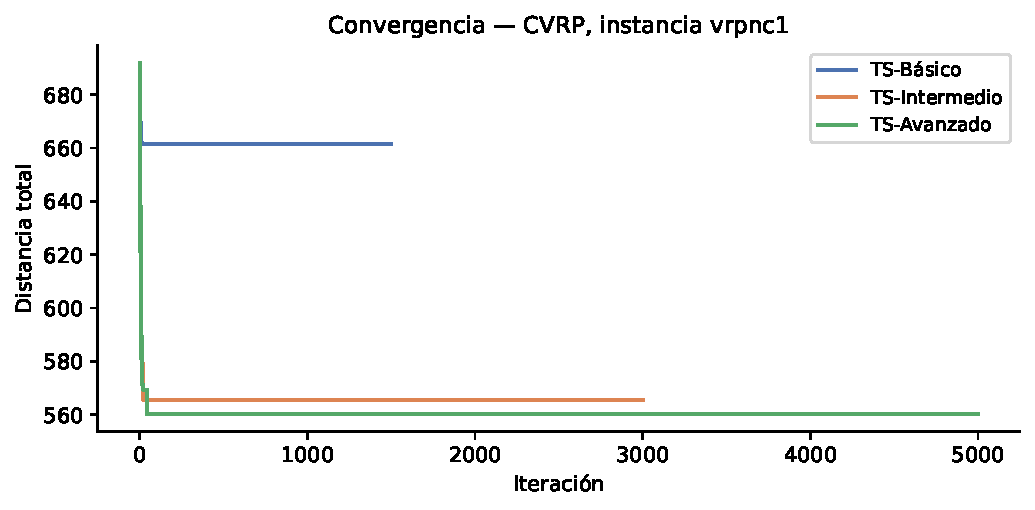
\includegraphics[width=\columnwidth]{figuras/convergencia_vrp.pdf}
  \caption{Convergencia del GAP (\%) — CVRP, instancia vrpnc1.}
  \label{fig:conv_vrp}
\end{figure}

Este es el problema donde la progresión de niveles tiene mayor impacto.
TS-Básico alcanza GAPs de hasta \SI{26.26}{\percent} en \texttt{vrpnc1},
reflejo de la dificultad de balancear rutas con un operador de reubicación
simple.
TS-Intermedio introduce intra-2opt inter-ruta, reduciendo el GAP promedio
a \SI{7.72}{\percent}.
TS-Avanzado añade frecuencia por cliente y penalización adaptativa, obteniendo
\SI{6.38}{\percent} promedio.
Para instancias grandes (\texttt{vrpnc3}, \texttt{vrpnc4}) el tiempo de
cómputo fue el principal limitante; con más iteraciones se esperaría mayor
mejora.
En particular, \texttt{vrpnc4} (150 clientes) presenta una inversión:
TS-Avanzado (\SI{9.16}{\percent}) no supera a TS-Intermedio (\SI{8.70}{\percent}),
posiblemente porque la penalización adaptativa sobrepondera clientes
muy visitados en instancias con alta densidad de rutas.
La Figura~\ref{fig:conv_vrp} evidencia las diferencias en velocidad y
profundidad de convergencia entre los tres niveles.

% ── Flowshop ────────────────────────────────────────────────────────────────
\subsection{Permutation Flowshop}

\begin{table}[t]
\caption{Resultados Flowshop: GAP\,(\%) y tiempo (s) — media(±$\sigma$) sobre 5 semillas}
\label{tab:flowshop}
\centering
\footnotesize
\setlength{\tabcolsep}{3pt}
\begin{tabular}{lcccccc}
\toprule
 & \multicolumn{3}{c}{\textbf{GAP (\%) $\bar{x}$($\pm\sigma$)}}
 & \multicolumn{3}{c}{\textbf{Tiempo (s) $\bar{x}$}} \\
\cmidrule{2-4}\cmidrule{5-7}
\textbf{Instancia} & B & I & A & B & I & A \\
\midrule
ta001 & 0.63(0.00) & 0.52(0.24) & 0.52(0.24)  &  0.84 &  1.72 &  1.88 \\
ta011 & 1.71(0.00) & 1.64(0.67) & 1.47(0.43)  &  1.30 &  2.85 &  3.75 \\
ta021 & 1.39(0.00) & 1.63(0.51) & 1.85(0.28)  &  2.74 &  5.68 &  6.30 \\
ta031 & 0.18(0.00) & 0.18(0.00) & 0.18(0.00)  &  4.78 &  9.68 & 11.91 \\
ta041 & 4.78(0.00) & 4.75(0.09) & 4.74(0.09)  &  9.01 & 17.55 & 21.80 \\
\midrule
\textbf{Media} & \textbf{1.74} & \textbf{1.74} & \textbf{1.75}
               & \textbf{3.73} & \textbf{7.50} & \textbf{9.13} \\
\bottomrule
\multicolumn{7}{l}{\scriptsize B=Básico, I=Intermedio, A=Avanzado. Formato: $\bar{x}$($\pm\sigma$)}
\end{tabular}
\end{table}

\begin{figure}[t]
  \centering
  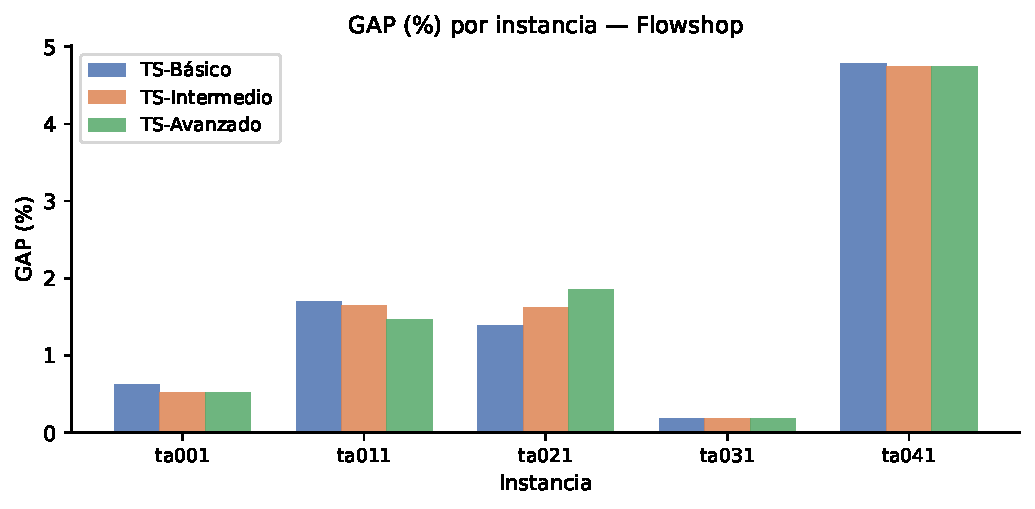
\includegraphics[width=\columnwidth]{figuras/convergencia_flowshop.pdf}
  \caption{GAP medio (\%) por instancia — Flowshop.}
  \label{fig:conv_flowshop}
\end{figure}

Los tres niveles obtienen GAPs medios muy similares:
\SI{1.74}{\percent}, \SI{1.74}{\percent} y \SI{1.75}{\percent}.
La heurística NEH entrega una solución inicial de buena calidad y la
vecindad de swap adyacente la mejora poco: los GAPs por instancia van de
\SI{0.18}{\percent} a \SI{4.78}{\percent}.
Para \texttt{ta041} (50 trabajos × 10 máquinas) el GAP se mantiene en
\SI{4.78}{\percent} para TS-Básico, \SI{4.75}{\percent} para TS-Intermedio y
\SI{4.74}{\percent} para TS-Avanzado; ello sugiere que la vecindad de swap
adyacente resulta limitada para explorar el espacio de búsqueda dentro del
presupuesto de iteraciones empleado; una vecindad de inserción podría
mejorar la solución a costa de tiempo computacional.
La Figura~\ref{fig:conv_flowshop} muestra el GAP medio por instancia: las
diferencias entre niveles son pequeñas y no siguen un orden fijo.
Los BKS de estas cinco instancias son makespan
óptimos~\cite{taillard1993benchmarks}; por ello, ningún GAP es negativo.
La Figura~\ref{fig:repr_soluciones} esquematiza cómo se representan las
soluciones que entrega cada algoritmo (archivo \texttt{solucion.txt} de
cada experimento).

\begin{figure}[t]
  \centering
  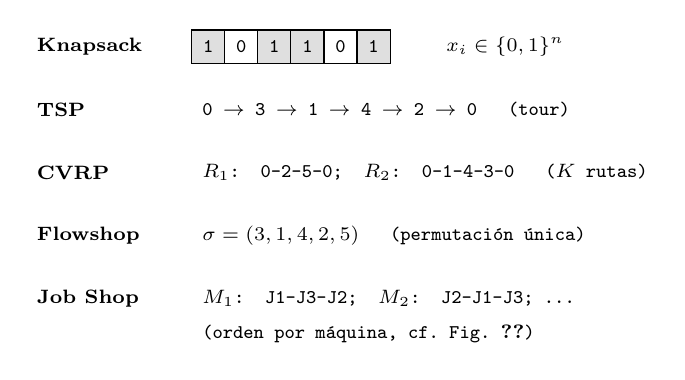
\begin{tikzpicture}[
      lab/.style={font=\scriptsize\bfseries, anchor=west},
      sol/.style={font=\scriptsize\ttfamily, anchor=west},
      celda/.style={draw, minimum width=0.42cm, minimum height=0.42cm,
                    font=\scriptsize\ttfamily, inner sep=1pt}]
    % Knapsack: vector binario
    \node[lab] at (0, 4.0) {Knapsack};
    \foreach \v/\i in {1/0, 0/1, 1/2, 1/3, 0/4, 1/5}
      \node[celda, fill={\ifnum\v=1 gray!25\else white\fi}]
        at (2.3 + \i*0.42, 4.0) {\v};
    \node[sol] at (5.2, 4.0) {$x_i \in \{0,1\}^n$};
    % TSP: tour
    \node[lab] at (0, 3.2) {TSP};
    \node[sol] at (2.1, 3.2)
      {0 $\to$ 3 $\to$ 1 $\to$ 4 $\to$ 2 $\to$ 0 \quad (tour)};
    % CVRP: rutas
    \node[lab] at (0, 2.4) {CVRP};
    \node[sol] at (2.1, 2.4)
      {$R_1$: 0-2-5-0;\ \ $R_2$: 0-1-4-3-0 \quad ($K$ rutas)};
    % Flowshop: permutación
    \node[lab] at (0, 1.6) {Flowshop};
    \node[sol] at (2.1, 1.6)
      {$\sigma = (3, 1, 4, 2, 5)$ \quad (permutación única)};
    % Job Shop: secuencia por máquina
    \node[lab] at (0, 0.8) {Job Shop};
    \node[sol] at (2.1, 0.8)
      {$M_1$: J1-J3-J2;\ \ $M_2$: J2-J1-J3;\ \ldots};
    \node[sol] at (2.1, 0.35)
      {(orden por máquina, cf.\ Fig.~\ref{fig:jobshop_gantt})};
  \end{tikzpicture}
  \caption{Representación de las soluciones en cada problema: vector
           binario (Knapsack), tour (TSP), conjunto de rutas (CVRP),
           permutación de trabajos (Flowshop) y orden de operaciones por
           máquina (Job Shop).}
  \label{fig:repr_soluciones}
\end{figure}

% ── Job Shop ────────────────────────────────────────────────────────────────
\subsection{Job Shop}

\begin{table}[t]
\caption{Resultados Job Shop: GAP\,(\%) y tiempo (s) — media(±$\sigma$) sobre 5 semillas}
\label{tab:jobshop}
\centering
\footnotesize
\setlength{\tabcolsep}{3pt}
\begin{tabular}{lcccccc}
\toprule
 & \multicolumn{3}{c}{\textbf{GAP (\%) $\bar{x}$($\pm\sigma$)}}
 & \multicolumn{3}{c}{\textbf{Tiempo (s) $\bar{x}$}} \\
\cmidrule{2-4}\cmidrule{5-7}
\textbf{Instancia} & B & I & A & B & I & A \\
\midrule
ft10 & 19.78(0.00) & 20.43(0.74) & 19.59(0.91)  &  8.49 &  3.11 &  4.53 \\
la01 & 1.80(0.00) & 2.25(1.24) & 1.65(0.57)  &  4.12 &  1.46 &  2.23 \\
la06 & 6.05(0.00) & 0.00(0.00) & 0.00(0.00)  & 13.28 &  4.73 &  6.91 \\
la11 & 0.00(0.00) & 1.33(1.57) & 0.00(0.00)  & 28.39 & 10.13 & 15.39 \\
la21 & 16.83(0.00) & 17.19(0.87) & 16.35(1.33)  & 25.98 & 10.12 & 14.34 \\
\midrule
\textbf{Media} & \textbf{8.89} & \textbf{8.24} & \textbf{7.52}
               & \textbf{16.05} & \textbf{5.91} & \textbf{8.68} \\
\bottomrule
\multicolumn{7}{l}{\scriptsize B=Básico, I=Intermedio, A=Avanzado. Formato: $\bar{x}$($\pm\sigma$)}
\end{tabular}
\end{table}

\begin{figure}[t]
  \centering
  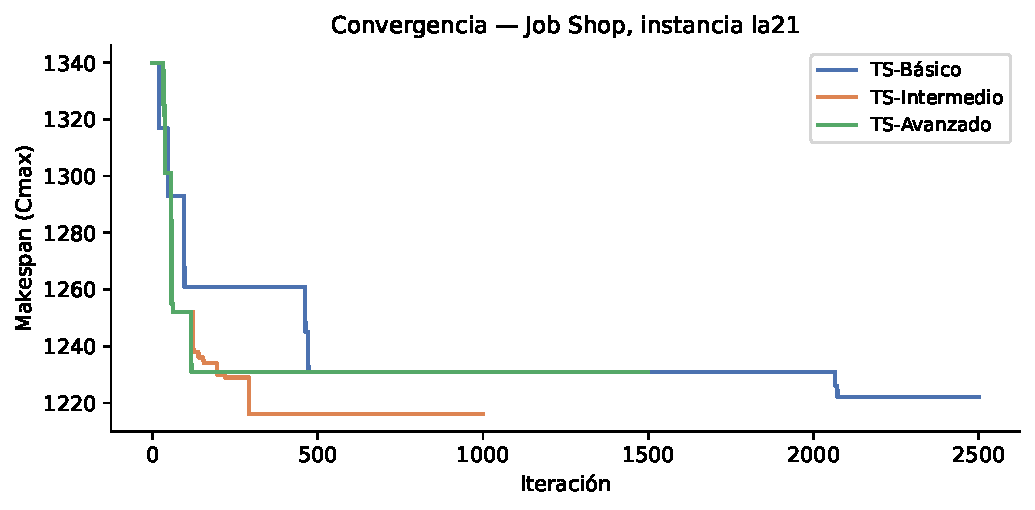
\includegraphics[width=\columnwidth]{figuras/convergencia_jobshop.pdf}
  \caption{Convergencia del GAP (\%) — Job Shop, instancia la21.}
  \label{fig:conv_jobshop}
\end{figure}

Job Shop es el problema más difícil del conjunto: \texttt{la21} y
\texttt{ft10} presentan GAPs de \SI{16.35}{\percent}–\SI{20.43}{\percent},
consistentes con la dificultad conocida de estos
benchmarks~\cite{nowicki1996fast}, y la
Figura~\ref{fig:conv_jobshop} confirma la estabilización temprana del GAP
en \texttt{la21}.
Las regresiones puntuales de TS-Intermedio (\texttt{la11}, \texttt{ft10})
y su alta varianza sugieren que la lista tabú dinámica y la penalización
de frecuencia son inestables en espacios de búsqueda muy accidentados.
En cambio, las instancias pequeñas (\texttt{la01}, \texttt{la06}) alcanzan
GAPs de \SI{0.00}{\percent}–\SI{2.25}{\percent}, al validar el decodificador
de Giffler-Thompson~\cite{giffler1960algorithms}.
TS-Intermedio es más rápido que TS-Básico ($5.91$\,s vs.\ $16.05$\,s)
porque emplea $T_{\max}=1\,000$ iteraciones frente a $2\,500$
(véase Tabla~\ref{tab:parametros}), decisión de diseño que mantiene tiempos
comparables dado el mayor costo por iteración de la lista dinámica.

% ── Análisis global ──────────────────────────────────────────────────────────
\subsection{Análisis global}

\begin{table}[tb]
\caption{GAP promedio (\%) y tiempo promedio (s) por problema y algoritmo}
\label{tab:consolidada}
\centering
\footnotesize
\setlength{\tabcolsep}{4pt}
\begin{tabular}{lcccccc}
\toprule
 & \multicolumn{2}{c}{\textbf{TS-Básico}}
 & \multicolumn{2}{c}{\textbf{TS-Intermedio}}
 & \multicolumn{2}{c}{\textbf{TS-Avanzado}} \\
\cmidrule{2-3}\cmidrule{4-5}\cmidrule{6-7}
\textbf{Problema} & GAP\% & T(s) & GAP\% & T(s) & GAP\% & T(s) \\
\midrule
Knapsack    & 0.22  & 0.01  & 0.13  & 0.02  & 0.10  & 0.07  \\
TSP         & 2.42  & 1.91  & 2.15  & 4.09  & 1.22  & 8.39  \\
CVRP        & 19.22  & 2.93  & 7.72  & 9.21  & 6.38  & 69.25  \\
Flowshop    & 1.74  & 3.73  & 1.74  & 7.50  & 1.75  & 9.13  \\
Job Shop    & 8.89  & 16.05  & 8.24  & 5.91  & 7.52  & 8.68  \\
\midrule
\textbf{Global} & \textbf{6.50} & -- & \textbf{4.00} & -- & \textbf{3.40} & -- \\
\bottomrule
\end{tabular}
\end{table}

El Cuadro~\ref{tab:consolidada} sintetiza los resultados a nivel de problema.
El costo computacional crece con el nivel, pero de forma moderada:
TS-Avanzado requiere en promedio $3.9\times$ el tiempo de TS-Básico,
mientras que la reducción de GAP es del \SI{48}{\percent} relativo.
